%!TEX root = report.tex

\chapter{The C3AE Model}
\label{chp:theorystuff}

\section{Model details}

The C3AE plain model takes as input a source image and tries to output a plausible estimation for the 
age of the portrayed person.

Since the objective is to obtain a lightweight model the total number of parameters needs to be as low 
as possible, as long as it doesn't affect the overall performance. 
For this reason the input image size is limited (64×64×3) and the other channels sizes are also small.\\
Standard convolutional layers are adequate for the trade-off between accuracy and compactness (as 
opposed to the separable convolution block used in the bigger models like MobileNets and ShuffleNets), 
followed by batch normalization, Relu and average pooling (BRA).\\
The model is composed of five of these standard convolutions and two fully connected layers as shown 
in \autoref{tab:architecture}.

\begin{center}
    \begin{tabular}{||c | c c c c||} 
    \hline
    Layer & Kernel & Stride & Output size & Parameters \\ 
    \hline\hline
    Image & - & 1 & 64×64×3 & - \\
    \hline
    Conv. 1 & 3×3×32 & 1 & 62×62×32 & 896 \\
    \hline
    BRA & - & 1 & 31×31×32 & 128 \\
    \hline
    Conv. 2 & 3×3×32 & 1 & 29×29×32 & 9248 \\
    \hline
    BRA & - & 1 & 14×14×32 & 128 \\ 
    \hline
    Conv. 3 & 3×3×32 & 1 & 12×12×32 & 9248 \\ 
    \hline
    BRA & - & 1 & 6×6×32 & 128 \\ 
    \hline
    Conv. 4 & 3×3×32 & 1 & 4×4×32 & 9248 \\ 
    \hline
    BN + ReLu & - & 1 & 4×4×32 & 128 \\ 
    \hline
    Conv5 & 1×1×32 & 1 & 4×4×32 & 1056 \\ 
    \hline
    Feat. & 1×1×32 & 1 & 12 & 6156 \\ 
    \hline
    Predict. & 1×1×1 & 1 & 1 & 13 \\ 
    \hline
    \end{tabular}
    \captionof{table}{Architecture of the model}
    \label{tab:architecture}
\end{center}

To estimate people's age C3AE considers two objectives simultaneously: the first one minimizes the 
Kullback-Leibler loss between distributions, and the second one optimizes the squared loss between 
discrete ages.

In the following sections are mentioned this and other techniques used in C3AE.

\begin{figure}[!ht]
    \centering
    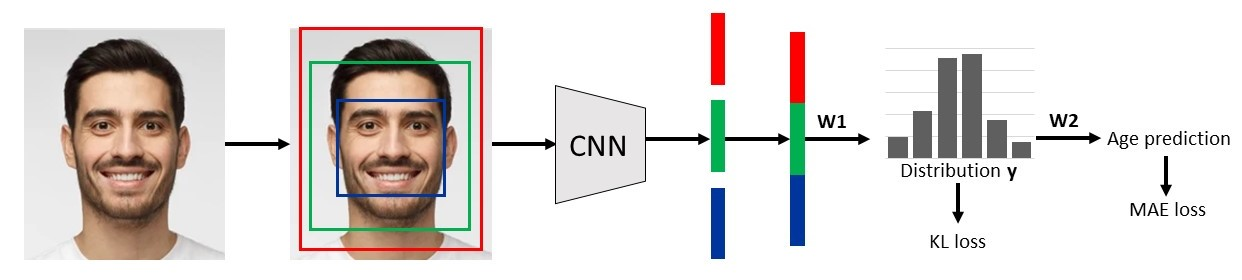
\includegraphics[width=400pt]{images/model.jpg}
    \caption{Overview of the model age estimation process}
    \label{fig:overview}
\end{figure}

\subsection*{Context-based Regression}
The resolution and the size of small-scale image is limited, so the idea is to exploit facial information 
at different granularity levels. 
After the face recognition task we identify three different crops of different sizes of the subject's face, 
like in Figure 3.1. Each cropped image has a special view on the face. 
The smaller image contains rich local information; in return the bigger one may contain global and scene 
information.
The three crops are then fed into the shared CNN network, and finally the bottlenecks of the
three-scale facial images are aggregated by concatenation.

\subsection*{Two-point Age Representation}
With C3AE we don't predict directly the age as a number. Instead, this model uses a two-point age 
representation through a distribution over two discrete adjacent bins.\\
For example let's consider the corresponding representation of an age of 22 with 10 bins. In this 
case the set of bins is [10, 20, 30, 40, 50, 60, 70, 80, 90, 100] and the corresponding vector 
representation of the age is [0, 0.8, 0.2, 0, 0, 0, 0, 0, 0, 0].

\subsection*{Cascade Training}
From the above section, the age value can be represented as a distribution vector. The mapping from this 
vector to age value is decomposed into two steps, where we define two different losses for the two cascade 
tasks.\\
The first one ($L_{kl}$) measures the discrepancy between ground-truth label and predicted age distribution.
We adopt KL-Divergence as the measurement.\\
The second loss ($L_{reg}$) controls the prediction of the final age and is implemented as an L1 distance
or mean absolute error (MAE loss).\\
In the training process the two loss functions are considered in the cascade style as shown in Figure 3.1 
but they are still trained jointly, and the total loss is given as
$L_{total} = \alpha L_{kl} + L_{reg}$, where $\alpha$ is the hyperparameter to balance the two losses.

\section{Implementation}
TODO